\documentclass[a4paper,12pt]{article}
\input{preambuleSLiCAP.tex}
\title{Use \LaTeX$\,$ as SLiCAP report generator}
\author{Anton J.M. Montagne}
\begin{document}
\maketitle
\tableofcontents
\newpage
\begin{abstract}
{\textbf{This document describes how to use \LaTeX$\,$ as SLiCAP report generator and
obtain documents with expressions, equations, figures, and tables all updated at document compilation.}}
\end{abstract}
\newpage

\section{Introduction}
Combining SLiCAP with \LaTeX$\,$ makes it possible to write technical reports while doing the design work.
Each time, before before document compilation, figures, tables, graphs, expressions and equations generated by SLiCAP are automatically updated and imported in the \LaTeX$\,$ source.

This document briefly describes the way of working. The \LaTeX$\,$source code of this document is {\texttt{tex/SLiCAP\_latex.tex}}; the path is relative to the SLiCAP project folder. The SLiCAP (Python) source code for this document is {\texttt{latexReport.py}}; in the SLiCAP project folder.

\subsection{Project file locations}\label{sec-project}

The project file locations are set and can be altered in the {\textbf{[projectpaths]}} section of the {\texttt{SLiCAP.ini}} file in the SLiCAP project folder. Below the listing of this section for this project:

\lstinputlisting[style=default, numbers=left, linerange={47-61}, firstnumber=47]{../SLiCAP.ini}

Below the relevant paths for making SLiCAP \LaTeX$\,$ reports. {\em{All paths are relative to the project folder; not shown, absolute path is listed in line 62:}} {\texttt{project=}}

\begin{itemize}
 \item {\texttt{cir}}: path to circuit netlist files, e.g. netlist files generated with {\texttt{makeCircuit()}}
 \item {\texttt{csv}}: path to {\texttt{.csv}} files, e.g. {\texttt{.csv}} files generated with {\texttt{specs2csv()}}
 \item {\texttt{tex\_snippets}}: path to \LaTeX$\,$ snippets generated by the \LaTeX$\,$ formatter.
 \item {\texttt{img}}: path to image files {\texttt{.svg, .png, .pdf, gif,} etc.}, e.g. generated with plot instructions and with {\texttt{makeCircuit()}}.
 \item {\texttt{tex}}: path to your \LaTeX$\,$ report files and to {\texttt{preambuleSLiCAP.tex}}.
\end{itemize}

\subsection{The preambule}
The file {\texttt{preambuleSLiCAP.tex}} imports packages, and defines colors and styles for SLiCAP. It must be imported at the beginning of the document, before {\textbf{$\backslash$begin\{document\}}}. Below you will find the opening of {\em{this}} document:

\lstinputlisting[style=latex, numbers=left, linerange={1-5} ]{SLiCAP\_latex.tex}

\section{SLiCAP creation of \LaTeX$\,$ output}

SLiCAP lets you create \LaTeX$\,$ output in two ways:

\begin{itemize}
\item Create images and code listings with SLiCAP functions

The generation and inclusion of images and code listings in \LaTeX$\,$ will be discussed in section \ref{sec-slicapfncts}.

\item Use the SLiCAP \LaTeX$\,$ formatter to produce \LaTeX$\,$ snippets

The generation and inclusion of \LaTeX$\,$ snippets using the formatter will be discussed in section \ref{sec-fmtmethods}.
\end{itemize}

\subsection{SLiCAP functions}\label{sec-slicapfncts}

In the next sections we will describe SLiCAP functions that generate data that can directly be imported by \LaTeX.

\subsubsection{\texttt{makeCircuit()}}

if KiCad or Lepton-EDA is used as schematic capture program, {\texttt{makeCircuit()}} creates drawing size images in {\texttt{.svg}} and {\texttt{.pdf}} format in the images folder (see section \ref{sec-project} for file locations).

\lstinputlisting[style=slicap, numbers=left, linerange={14-15}, firstnumber=14]{../LaTeXreport.py}

The \LaTeX$\,$ code to include the schematic circuit diagram of {\texttt{cir}} is:

\lstinputlisting[style=latex, numbers=left, linerange={72-78}, firstnumber=72]{SLiCAP\_latex.tex}

The result is shown in Figure \ref{fig-myPassiveNetwork}.

\begin{figure}[h]
\centering
 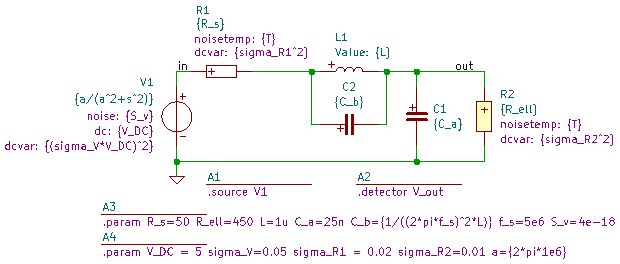
\includegraphics[width=16cm]{../img/myPassiveNetwork.pdf}
 \caption{Schematic diagram}
 \label{fig-myPassiveNetwork}
\end{figure}

The netlist file that is created with {\texttt{makeCircuit()}} can be displayed in the \LaTeX$\,$ document using:

\lstinputlisting[style=latex, numbers=left, linerange={85}, firstnumber=85]{SLiCAP\_latex.tex}

This will render as follows:

\lstinputlisting[language=ltspice, numbers=left]{../cir/myPassiveNetwork.cir}

\subsubsection{plot(), plotSweep(), and plotPZ()}

Figure \ref{fig-dBmag} shows the {\texttt{dBmag}} plot of the source-to-load transfer of the circuit.

\begin{figure}[h]
\centering
 \includegraphics[width=12cm]{../img/dBmag.pdf}
 \caption{Magnitude plot of the source-to-load transfer}
 \label{fig-dBmag}
\end{figure}

The SLiCAP code for creating this plot is:

\lstinputlisting[style=slicap, numbers=left, linerange={69-72}, firstnumber=69]{../LaTeXreport.py}

The \LaTeX$\,$ source for including it is:

\lstinputlisting[style=latex, numbers=left, linerange={91-96}, firstnumber=91]{SLiCAP\_latex.tex}

\subsection{\LaTeX$\,$ formatter}\label{sec-fmtmethods}

The \LaTeX$\,$ formatter in SLiCAP generates \LaTeX$\,$ snippets that can be imported in \LaTeX$\,$ documents using {\textbf{$\backslash$input\{\}}} statements. It needs to be initialized. An example of the initialization of this formatter is shown below (see line 12).

\lstinputlisting[style=slicap, numbers=left, linerange={8-12}, firstnumber=8 ]{../LaTeXreport.py}

In the following sections we describe formatter methods (in aplhabetic order) that generate specific \LaTeX$\,$ snippets.

\subsubsection{\texttt{coeffsTransfer(transferCoeffs, label="", caption="", \\ color="myyellow")}}

This method is used to display the numerator and denominator coefficients of a rational function in the form of a table.

Let $H(s)=$%
\input{SLiCAPdata/H2.tex}.

Table \ref{tab-coeffs} shows the numerator and denominator coefficients of the Laplace variable $s$ of $H(s)$.

\begin{table}[H]
\centering
\begin{tabular}[c]{ll}
\textbf{Coeff} & \textbf{Value} \\ 
\rowcolor{myyellow}
$b_{\mathrm{0}}$ &$R_{\ell}$ \\ 
$b_{\mathrm{1}}$ &$0$ \\ 
\rowcolor{myyellow}
$b_{\mathrm{2}}$ &$C_{\mathrm{b}} L R_{\ell}$ \\ 
$a_{\mathrm{0}}$ &$R_{\ell} + R_{\mathrm{s}}$ \\ 
\rowcolor{myyellow}
$a_{\mathrm{1}}$ &$C_{\mathrm{a}} R_{\ell} R_{\mathrm{s}} + L$ \\ 
$a_{\mathrm{2}}$ &$L \left(C_{\mathrm{a}} R_{\ell} + C_{\mathrm{b}} R_{\ell} + C_{\mathrm{b}} R_{\mathrm{s}}\right)$ \\ 
\rowcolor{myyellow}
$a_{\mathrm{3}}$ &$C_{\mathrm{a}} C_{\mathrm{b}} L R_{\ell} R_{\mathrm{s}}$ \\ 
\end{tabular}
\caption{Numerator and denominator coefficients of $H(s)$, $b_i$ and $a_i$, respectively}
\label{tab-coeffs}
\end{table}



SLiCAP script:

\lstinputlisting[style=slicap, numbers=left, linerange={57-67}, firstnumber=57]{../LaTeXreport.py}

\LaTeX$\,$ code:

\lstinputlisting[style=latex, numbers=left, linerange={123}, firstnumber=123]{SLiCAP\_latex.tex}

\subsubsection{\texttt{dcvarContribs(resultObject, label="", caption="", \\ color="myyellow")}}

The individual contributions of independent DC error sources to the detector-referred and source-referred dc variance can be exported in the form of a \LaTeX$\,$ table.

SLiCAP code:

\lstinputlisting[style=slicap, numbers=left, linerange={74-76}, firstnumber=74]{../LaTeXreport.py}

\LaTeX$\,$ code:

\lstinputlisting[style=latex, numbers=left, linerange={147}, firstnumber=147]{SLiCAP\_latex.tex}

The result is shown in Table \ref{tab-dcvar}.

\begin{table}[H]
\centering
\begin{tabular}[c]{lll}
\textbf{Name} & \textbf{Value} & \textbf{Units} \\ 
\rowcolor{myyellow}
\small{V1: Value} &$V_{\mathrm{DC}}^{2} \sigma_{\mathrm{V}}^{2}$ &$\mathrm{V^2}$ \\ 
\small{V1: Source-referred} &$V_{\mathrm{DC}}^{2} \sigma_{\mathrm{V}}^{2} \left(C_{\mathrm{b}} L s^{2} + 1\right)^{2}$ &$\mathrm{V^2}$ \\ 
\rowcolor{myyellow}
\small{V1: Detector-referred} &$\frac{R_{\ell}^{2} V_{\mathrm{DC}}^{2} \sigma_{\mathrm{V}}^{2} \left(C_{\mathrm{b}} L s^{2} + 1\right)^{2}}{\left(R_{\ell} + R_{\mathrm{s}}\right)^{2}}$ &$\mathrm{V^2}$ \\ 
\small{I\_dcvar\_R1: Value} &$\frac{V_{\mathrm{DC}}^{2} \sigma_{\mathrm{R1}}^{2}}{\left(R_{\ell} + R_{\mathrm{s}}\right)^{2}}$ &$\mathrm{A^2}$ \\ 
\rowcolor{myyellow}
\small{I\_dcvar\_R1: Source-referred} &$\frac{R_{\mathrm{s}}^{2} V_{\mathrm{DC}}^{2} \sigma_{\mathrm{R1}}^{2}}{\left(R_{\ell} + R_{\mathrm{s}}\right)^{2}}$ &$\mathrm{V^2}$ \\ 
\small{I\_dcvar\_R1: Detector-referred} &$\frac{R_{\ell}^{2} R_{\mathrm{s}}^{2} V_{\mathrm{DC}}^{2} \sigma_{\mathrm{R1}}^{2}}{\left(R_{\ell} + R_{\mathrm{s}}\right)^{4}}$ &$\mathrm{V^2}$ \\ 
\rowcolor{myyellow}
\small{I\_dcvar\_R2: Value} &$\frac{V_{\mathrm{DC}}^{2} \sigma_{\mathrm{R2}}^{2}}{\left(R_{\ell} + R_{\mathrm{s}}\right)^{2}}$ &$\mathrm{A^2}$ \\ 
\small{I\_dcvar\_R2: Source-referred} &$\frac{R_{\mathrm{s}}^{2} V_{\mathrm{DC}}^{2} \sigma_{\mathrm{R2}}^{2}}{\left(R_{\ell} + R_{\mathrm{s}}\right)^{2}}$ &$\mathrm{V^2}$ \\ 
\rowcolor{myyellow}
\small{I\_dcvar\_R2: Detector-referred} &$\frac{R_{\ell}^{2} R_{\mathrm{s}}^{2} V_{\mathrm{DC}}^{2} \sigma_{\mathrm{R2}}^{2}}{\left(R_{\ell} + R_{\mathrm{s}}\right)^{4}}$ &$\mathrm{V^2}$ \\ 
\end{tabular}
\caption{dcvar analysis results}
\label{tab-dcvar}
\end{table}



\subsubsection{\texttt{dictTable(dct, head=None, label="", caption="", \\ color=myyellow")}}

This method displays the key-value pairs of a dictionary in the form of a table.

SLiCAP code:

\lstinputlisting[style=slicap, numbers=left, linerange={49-55}, firstnumber=49]{../LaTeXreport.py}

\LaTeX$\,$ code:

\lstinputlisting[style=latex, numbers=left, linerange={163}, firstnumber=163]{SLiCAP\_latex.tex}

The result is shown in Table \ref{tab-mydct}.  Please notice the change of the default alternate row color as specified in line 52 of the SLiCAP script above.

\begin{table}[H]
\centering
\begin{tabular}[c]{ll}
\textbf{Name} & \textbf{Value} \\ 
\rowcolor{mygray}
$R_{\mathrm{s}}$ &$150$ \\ 
$R_{\ell}$ &$50$ \\ 
\rowcolor{mygray}
$L$ &$1.0 \cdot 10^{-6}$ \\ 
$C_{\mathrm{a}}$ &$2.5 \cdot 10^{-8}$ \\ 
\rowcolor{mygray}
$C_{\mathrm{b}}$ &$2.5 \cdot 10^{-10}$ \\ 
$S_{\mathrm{v}}$ &$4.0 \cdot 10^{-18}$ \\ 
\rowcolor{mygray}
$V_{\mathrm{DC}}$ &$5$ \\ 
$\sigma_{\mathrm{V}}$ &$0.05$ \\ 
\rowcolor{mygray}
$\sigma_{\mathrm{R1}}$ &$0.02$ \\ 
$\sigma_{\mathrm{R2}}$ &$0.01$ \\ 
\rowcolor{mygray}
$T$ &$300$ \\ 
\end{tabular}
\caption{Circuit parameters using the dictTable format and modified alternate row color.}
\label{tab-mydct}
\end{table}



\subsubsection{\texttt{elementData(circuitObject, label="", caption="")}}

This method displays the expanded netlist of a circuit object in the form of a table.

SLiCAP code:

\lstinputlisting[style=slicap, numbers=left, linerange={19,20}, firstnumber=19]{../LaTeXreport.py}

\LaTeX$\,$ code:

\lstinputlisting[style=latex, numbers=left, linerange={177-179}, firstnumber=177]{SLiCAP\_latex.tex}

Table \ref{tab-expanded} shows the result.

\begin{table}[H]
\centering
\begin{tabular}[c]{lllllll}
\textbf{ID} & \textbf{Nodes} & \textbf{Refs} & \textbf{Model} & \textbf{Param} & \textbf{Symbolic} & \textbf{Numeric} \\ 
\rowcolor{myyellow}
\small{C1} &\small{0 out } & &\small{C} &\small{value} &$C_{\mathrm{a}}$ &$2.5 \cdot 10^{-8}$ \\ 
 & & & &\small{vinit} &$0$ &$0$ \\ 
\rowcolor{myyellow}
\small{C2} &\small{out 1 } & &\small{C} &\small{value} &$C_{\mathrm{b}}$ &$2.5 \cdot 10^{-10}$ \\ 
 & & & &\small{vinit} &$0$ &$0$ \\ 
\rowcolor{myyellow}
\small{L1} &\small{1 out } & &\small{L} &\small{value} &$L$ &$1.0 \cdot 10^{-6}$ \\ 
 & & & &\small{iinit} &$0$ &$0$ \\ 
\rowcolor{myyellow}
\small{R1} &\small{1 in } & &\small{R} &\small{value} &$R_{\mathrm{s}}$ &$150$ \\ 
 & & & &\small{noisetemp} &$T$ &$300$ \\ 
\rowcolor{myyellow}
 & & & &\small{noiseflow} &$0$ &$0$ \\ 
 & & & &\small{dcvar} &$\sigma_{\mathrm{R1}}^{2}$ &$0.0004$ \\ 
\rowcolor{myyellow}
 & & & &\small{dcvarlot} &$0$ &$0$ \\ 
\small{R2} &\small{out 0 } & &\small{R} &\small{value} &$R_{\ell}$ &$50$ \\ 
\rowcolor{myyellow}
 & & & &\small{noisetemp} &$T$ &$300$ \\ 
 & & & &\small{noiseflow} &$0$ &$0$ \\ 
\rowcolor{myyellow}
 & & & &\small{dcvar} &$\sigma_{\mathrm{R2}}^{2}$ &$0.0001$ \\ 
 & & & &\small{dcvarlot} &$0$ &$0$ \\ 
\rowcolor{myyellow}
\small{V1} &\small{in 0 } & &\small{V} &\small{value} &$\frac{1}{s}$ &$\frac{1}{s}$ \\ 
 & & & &\small{noise} &$S_{\mathrm{v}}$ &$4.0 \cdot 10^{-18}$ \\ 
\rowcolor{myyellow}
 & & & &\small{dc} &$V_{\mathrm{DC}}$ &$5$ \\ 
 & & & &\small{dcvar} &$V_{\mathrm{DC}}^{2} \sigma_{\mathrm{V}}^{2}$ &$0.0625$ \\ 
\end{tabular}
\caption{Expanded netlist}
\label{tab-expanded}
\end{table}



\subsubsection{\texttt{eqn(LHS, RHS, units="", label="", multiline=False)}}

The formatter method {\texttt{eqn()}} creates a \LaTeX$\,$ snippet of a displayed and numbered equation.

SLiCAP code:

\lstinputlisting[style=slicap, numbers=left, linerange={37-41}, firstnumber=37]{../LaTeXreport.py}

\LaTeX$\,$ code:

\lstinputlisting[style=latex, numbers=left, linerange={195-196}, firstnumber=195]{SLiCAP\_latex.tex}

This renders as:

The transfer function is shown in (\ref{eq-H1}).
\input{SLiCAPdata/H1.tex}

If {\texttt{multiline=True}} SLiCAP breaks the equation in parts of a sum or a product.

\subsubsection{\texttt{eqnInline(LHS, RHS, units="")}}

The method {\texttt{eqnInline()}} produces a \LaTeX$\,$ snippet for an inline equation.

SLiCAP code:

\lstinputlisting[style=slicap, numbers=left, linerange={46-47}, firstnumber=46]{../LaTeXreport.py}

\LaTeX$\,$ code:

\lstinputlisting[style=latex, numbers=left, linerange={214-215}, firstnumber=214]{SLiCAP\_latex.tex}

This renders as:

You can write (\ref{eq-H1}) inline as:
$\frac{V_{\mathrm{out}}}{V_{\mathrm{in}}}=\frac{R_{\ell} \left(C_{\mathrm{b}} L s^{2} + 1\right)}{\left(R_{\ell} + R_{\mathrm{s}}\right) \left(\frac{C_{\mathrm{a}} C_{\mathrm{b}} L R_{\ell} R_{\mathrm{s}} s^{3}}{R_{\ell} + R_{\mathrm{s}}} + \frac{s^{2} \left(C_{\mathrm{a}} L R_{\ell} + C_{\mathrm{b}} L R_{\ell} + C_{\mathrm{b}} L R_{\mathrm{s}}\right)}{R_{\ell} + R_{\mathrm{s}}} + \frac{s \left(C_{\mathrm{a}} R_{\ell} R_{\mathrm{s}} + L\right)}{R_{\ell} + R_{\mathrm{s}}} + 1\right)}$ .

\subsubsection{\texttt{expr(expr, units="")}}

The method {\texttt{expr()}} creates a \LaTeX$\,$ snippet of an inline expression.

SLiCAP code:

\lstinputlisting[style=slicap, numbers=left, linerange={43-44}, firstnumber=43]{../LaTeXreport.py}

\LaTeX$\,$ code:

\lstinputlisting[style=latex, numbers=left, linerange={231-232}, firstnumber=231]{SLiCAP\_latex.tex}

This renders as:

The transfer can be written as:
\input{SLiCAPdata/H2.tex}.

\subsubsection{\texttt{file(fileName, lineRange=None, firstNumber=None, language=None, \\ style=None)}}

The method {\texttt{file()}} generates a \LaTeX$\,$ snippet for displaying a code file. The keyword {\texttt{language}} overrides {\texttt{style}}. SLiCAP built-in styles can be seen in {\texttt{preambule.tex}}.

SLiCAP code:

\lstinputlisting[style=slicap, numbers=left, linerange={92}, firstnumber=92]{../LaTeXreport.py}

Please notice the file path relative to the \LaTeX$\,$ document.

\LaTeX$\,$ code:

\lstinputlisting[style=latex, numbers=left, linerange={250}, firstnumber=250]{SLiCAP\_latex.tex}

This renders as:

{\textbf{File:} myPassiveNetwork.cir}

\lstinputlisting[language=ltspice, numbers=left]{../cir/myPassiveNetwork.cir}



\subsubsection{\texttt{matrixEqn(Iv, M, Dv, label="")}}

The method {\texttt{matrixEqn()}} generates a \LaTeX$\,$ snippet for a displayed matrix equation.
\texttt{Iv}, \texttt{M}, and \texttt{Dv} must be Sympy matrices, representing the vector with independent variables, the transfer matrix, and the vector with dependent variables, respectively.

SLiCAP code:

\lstinputlisting[style=slicap, numbers=left, linerange={28-35}, firstnumber=28]{../LaTeXreport.py}

\LaTeX$\,$ code:

\lstinputlisting[style=latex, numbers=left, linerange={267-268}, firstnumber=267]{SLiCAP\_latex.tex}

This renders as:

The matrix equation of the network is given in (\ref{eq-matrices}).
\begin{equation}
\left[\begin{matrix}0\\\frac{1}{s}\\0\\0\\0\end{matrix}\right]=\left[\begin{matrix}- L s & 0 & 1 & 0 & -1\\0 & 0 & 0 & 1 & 0\\1 & 0 & C_{\mathrm{b}} s + \frac{1}{R_{\mathrm{s}}} & - \frac{1}{R_{\mathrm{s}}} & - C_{\mathrm{b}} s\\0 & 1 & - \frac{1}{R_{\mathrm{s}}} & \frac{1}{R_{\mathrm{s}}} & 0\\-1 & 0 & - C_{\mathrm{b}} s & 0 & C_{\mathrm{a}} s + C_{\mathrm{b}} s + \frac{1}{R_{\ell}}\end{matrix}\right]\cdot \left[\begin{matrix}I_{\mathrm{L1}}\\I_{\mathrm{V1}}\\V_{\mathrm{1}}\\V_{\mathrm{in}}\\V_{\mathrm{out}}\end{matrix}\right]
\label{eq-matrices}
\end{equation}



\subsubsection{\texttt{netlist(netlistFile, lineRange=None, firstNumber=None)}}

This method creates an $\backslash${\textbf{input\{\}}} statement for a SLiCAP netlist file.

SLiCAP code:

\lstinputlisting[style=slicap, numbers=left, linerange={15-18}, firstnumber=15]{../LaTeXreport.py}

\LaTeX$\,$ code:

\lstinputlisting[style=latex, numbers=left, linerange={284}, firstnumber=284]{SLiCAP\_latex.tex}

This renders as:

\textbf{Netlist: myPassiveNetwork.cir}

\lstinputlisting[language=ltspice, numbers=left]{/home/anton/DATA/SLiCAP/SLiCAP_python_tests/FilterDesign/cir/myPassiveNetwork.cir}



\subsubsection{\texttt{noiseContribs(resultObject, label="", caption="", \\ color="myyellow")}}

The method {\texttt{noiseContribs()}} creates a table with noise sources and their contributions to the source-referred noise and the detector-referred noise.

SLiCAP code:

\lstinputlisting[style=slicap, numbers=left, linerange={78-79}, firstnumber=78]{../LaTeXreport.py}

\LaTeX$\,$ code:

\lstinputlisting[style=latex, numbers=left, linerange={300}, firstnumber=300]{SLiCAP\_latex.tex}

This renders as shown in Table \ref{tab-noise}.

\begin{table}[H]
\centering
\begin{tabular}[c]{lll}
\textbf{Name} & \textbf{Value} & \textbf{Units} \\ 
\rowcolor{myyellow}
\small{V1: Value} &$4.0 \cdot 10^{-18}$ &$\mathrm{\frac{V^2}{Hz}}$ \\ 
\small{V1: Source-referred} &$4.0 \cdot 10^{-18}$ &$\mathrm{\frac{V^2}{Hz}}$ \\ 
\rowcolor{myyellow}
\small{V1: Detector-referred} &$\frac{6.4 \cdot 10^{23} \left(9.87 \cdot 10^{-15} f^{2} - 1\right)^{2}}{8653.0 f^{6} - 1.594 \cdot 10^{18} f^{4} + 8.846 \cdot 10^{31} f^{2} + 2.56 \cdot 10^{42}}$ &$\mathrm{\frac{V^2}{Hz}}$ \\ 
\small{I\_noise\_R1: Value} &$1.105 \cdot 10^{-22}$ &$\mathrm{\frac{A^2}{Hz}}$ \\ 
\rowcolor{myyellow}
\small{I\_noise\_R1: Source-referred} &$2.485 \cdot 10^{-18}$ &$\mathrm{\frac{V^2}{Hz}}$ \\ 
\small{I\_noise\_R1: Detector-referred} &$\frac{3.976 \cdot 10^{23} \left(9.87 \cdot 10^{-15} f^{2} - 1\right)^{2}}{8653.0 f^{6} - 1.594 \cdot 10^{18} f^{4} + 8.846 \cdot 10^{31} f^{2} + 2.56 \cdot 10^{42}}$ &$\mathrm{\frac{V^2}{Hz}}$ \\ 
\rowcolor{myyellow}
\small{I\_noise\_R2: Value} &$3.314 \cdot 10^{-22}$ &$\mathrm{\frac{A^2}{Hz}}$ \\ 
\small{I\_noise\_R2: Source-referred} &$\frac{8.284 \cdot 10^{-49} \left(876.7 f^{4} - 1.619 \cdot 10^{17} f^{2} + 9.0 \cdot 10^{30}\right)}{\left(9.87 \cdot 10^{-15} f^{2} - 1\right)^{2}}$ &$\mathrm{\frac{V^2}{Hz}}$ \\ 
\rowcolor{myyellow}
\small{I\_noise\_R2: Detector-referred} &$\frac{1.325 \cdot 10^{-7} \left(876.7 f^{4} - 1.619 \cdot 10^{17} f^{2} + 9.0 \cdot 10^{30}\right)}{8653.0 f^{6} - 1.594 \cdot 10^{18} f^{4} + 8.846 \cdot 10^{31} f^{2} + 2.56 \cdot 10^{42}}$ &$\mathrm{\frac{V^2}{Hz}}$ \\ 
\end{tabular}
\caption{Noise contributions}
\label{tab-noise}
\end{table}



\subsubsection{\texttt{params(circuitObject, label="", caption="", color="myyellow")}}

This method creates a single-column table with names of undefined parameters.

SLiCAP code:

\lstinputlisting[style=slicap, numbers=left, linerange={25-26}, firstnumber=25]{../LaTeXreport.py}

\LaTeX$\,$ code:

\lstinputlisting[style=latex, numbers=left, linerange={316-318}, firstnumber=316]{SLiCAP\_latex.tex}

This renders as:

Undefined parameters are given in Table \ref{tab-params}

{\textbf{No undefined parameters in: myPassiveNetwork}}



\subsubsection{\texttt{parDefs(circuitObject, label="", caption="", color="myyellow")}}

This method creates a single-column table with circuit parameter definitions.

SLiCAP code:

\lstinputlisting[style=slicap, numbers=left, linerange={22-23}, firstnumber=22]{../LaTeXreport.py}

\LaTeX$\,$ code:

\lstinputlisting[style=latex, numbers=left, linerange={334-336}, firstnumber=334]{SLiCAP\_latex.tex}

This renders as:

Parameter definitions are given in Table \ref{tab-pardefs}

\input{SLiCAPdata/pardefs}

\subsubsection{\texttt{pz(resultObject, label="", append2caption="", \\ color="myyellow")}}

This method creates \LaTeX$\,$ table snippets for results of pole-zero analysis results.

SLiCAP code:

\lstinputlisting[style=slicap, numbers=left, linerange={81-90}, firstnumber=81]{../LaTeXreport.py}

\LaTeX$\,$ code for the poles table:

\lstinputlisting[style=latex, numbers=left, linerange={352-354}, firstnumber=352]{SLiCAP\_latex.tex}

This renders as:

The numeric poles are listed in Table \ref{tab-poles}.

\input{SLiCAPdata/poles.tex}

\LaTeX$\,$ code for the symbolic zeros table:

\lstinputlisting[style=latex, numbers=left, linerange={362-364}, firstnumber=362]{SLiCAP\_latex.tex}

This renders as:

The symbolic zeros are listed in Table \ref{tab-symzeros}.

\begin{table}[H]
\centering
\begin{tabular}[c]{ll}
\textbf{\#} & \textbf{f [Hz]} \\ 
\rowcolor{myyellow}
$z_{\mathrm{1}}$ &\small{$- \frac{0.5 \left(- \frac{1}{C\_{\mathrm{b}} L}\right)^{0.5}}{\pi}$} \\ 
$z_{\mathrm{2}}$ &\small{$\frac{0.5 \left(- \frac{1}{C\_{\mathrm{b}} L}\right)^{0.5}}{\pi}$} \\ 
\end{tabular}
\caption{Symbolic zeros of the transfer}
\label{tab-symzeros}
\end{table}



\LaTeX$\,$ code for the numeric zeros table:

\lstinputlisting[style=latex, numbers=left, linerange={372-374}, firstnumber=372]{SLiCAP\_latex.tex}

This renders as:

The numeric zeros are listed in Table \ref{tab-zeros}.

\begin{table}[H]
\centering
\begin{tabular}[c]{lrrrrr}
\textbf{\#} & \textbf{Re [Hz]} & \textbf{Im [Hz]} & \textbf{f [Hz]} & \textbf{Q} \\ 
\rowcolor{myyellow}
$z_{\mathrm{1}}$ &$0$ &$1.007 \cdot 10^{7}$ &$1.007 \cdot 10^{7}$ &$\tilde{\infty}$ \\ 
$z_{\mathrm{2}}$ &$0$ &$-1.007 \cdot 10^{7}$ &$1.007 \cdot 10^{7}$ &$\tilde{\infty}$ \\ 
\end{tabular}
\caption{Zeros of the transfer}
\label{tab-zeros}
\end{table}



\LaTeX$\,$ code for the numeric poles-zeros table:

\lstinputlisting[style=latex, numbers=left, linerange={382-387}, firstnumber=380]{SLiCAP\_latex.tex}

This renders as:

The poles and zeros are listed in Table \ref{tab-pz}.

\begin{table}[H]
\centering
\begin{tabular}[c]{lrrrrr}
\textbf{\#} & \textbf{Re [Hz]} & \textbf{Im [Hz]} & \textbf{f [Hz]} & \textbf{Q} \\ 
\rowcolor{myyellow}
$p_{\mathrm{1}}$ &$-1.701 \cdot 10^{5}$ &$0$ &$1.701 \cdot 10^{5}$ \\ 
$p_{\mathrm{2}}$ &$-2.122 \cdot 10^{6}$ &$9.83 \cdot 10^{6}$ &$1.006 \cdot 10^{7}$ &$2.37$ \\ 
\rowcolor{myyellow}
$p_{\mathrm{3}}$ &$-2.122 \cdot 10^{6}$ &$-9.83 \cdot 10^{6}$ &$1.006 \cdot 10^{7}$ &$2.37$ \\ 
\small{ } \\ 
\rowcolor{myyellow}
$z_{\mathrm{1}}$ &$0$ &$1.007 \cdot 10^{7}$ &$1.007 \cdot 10^{7}$ &$\tilde{\infty}$ \\ 
$z_{\mathrm{2}}$ &$0$ &$-1.007 \cdot 10^{7}$ &$1.007 \cdot 10^{7}$ &$\tilde{\infty}$ \\ 
\end{tabular}
\caption{Poles and zeros of the transfer}
\label{tab-pz}
\end{table}



The DC value of the transfer equals:
\input{SLiCAPdata/dcValue.tex}.

\subsubsection{\texttt{specs(specs, specType, label="", caption="", color="myyellow")}}

This method exprots a \LaTeX$\,$ snippet for a specification tabel.

SLiCAP code:

\lstinputlisting[style=slicap, numbers=left, linerange={94-102}, firstnumber=94]{../LaTeXreport.py}

\LaTeX$\,$ code for the performance specifications table:

\lstinputlisting[style=latex, numbers=left, linerange={403-405}, firstnumber=403]{SLiCAP\_latex.tex}

This renders as:

The performance specifications are listed in Table \ref{tab-performance}.

\begin{table}[H]
\centering
\begin{tabular}[c]{llrl}
\textbf{name} & \textbf{description} & \textbf{value} & \textbf{units} \\ 
\rowcolor{myyellow}
$f_{\mathrm{min}}$ &\small{Lower limit noise bandwidth} &$10$ &$\mathrm{Hz}$ \\ 
$f_{\mathrm{max}}$ &\small{Upper limit noise bandwidth} &$1.0 \cdot 10^{7}$ &$\mathrm{Hz}$ \\ 
\end{tabular}
\caption{Performance specifications}
\label{tab-performance}
\end{table}




\LaTeX$\,$ code for the design specifications table:

\lstinputlisting[style=latex, numbers=left, linerange={413-415}, firstnumber=413]{SLiCAP\_latex.tex}

This renders as:

The design specifications are listed in Table \ref{tab-design}.

\begin{table}[H]
\centering
\begin{tabular}[c]{llrl}
\textbf{name} & \textbf{description} & \textbf{value} & \textbf{units} \\ 
\rowcolor{myyellow}
$v_{\mathrm{n}}$ &\small{RMS output noise over noise bandwidth} &$4.558 \cdot 10^{-7}$ &$\mathrm{V}$ \\ 
\end{tabular}
\caption{Design specifications}
\label{tab-design}
\end{table}




\subsubsection{\texttt{stepArray(stepVars, stepArray, label="", caption="", \\ color="myyellow")}}

This method exports a \LaTeX$\,$ table snippet with step-data for array-type stepping.

SLiCAP code:

\lstinputlisting[style=slicap, numbers=left, linerange={104-112}, firstnumber=94]{../LaTeXreport.py}

\LaTeX$\,$ code for the step array table:

\lstinputlisting[style=latex, numbers=left, linerange={438-440}, firstnumber=438]{SLiCAP\_latex.tex}

\begin{figure}[H]
\centering
 \includegraphics[width=12cm]{../img/dBmagStepped.pdf}
 \caption{Magnitude plot of the source-to-load transfer}
 \label{fig-dBmagStepped}
\end{figure}

This renders as:

The step values that apply to Figure \ref{fig-dBmagStepped} are shown in Table \ref{tab-stepdict}.

\begin{table}[H]
\centering
\begin{tabular}[c]{lll}
\textbf{ } & $\mathbf{C_{\mathrm{b}}}$ & $\mathbf{R_{\ell}}$ \\ 
\rowcolor{myyellow}
\small{Run 1:} &$1.0 \cdot 10^{-10}$ &$150$ \\ 
\small{Run 2:} &$2.5 \cdot 10^{-10}$ &$100$ \\ 
\rowcolor{myyellow}
\small{Run 3:} &$5.0 \cdot 10^{-10}$ &$50$ \\ 
\end{tabular}
\caption{Step array}
\label{tab-stepdict}
\end{table}



\section{Change style}

Some publishers require authors to provide material formatted in predefined styles. There are different ways to format \LaTeX$\,$ snippets created with SLiCAP:

\begin{enumerate}
 \item Colors of code listings can be changed in the \LaTeX$\,$ preambule file
 \item If alternate row colors in tables are not desired, use {\texttt{color=white}} in formatter methods that create tables.
 \item If specific formatting of table captions is required, use {\texttt{caption=''}} and {\texttt{label=''}} in formatter methods that create tables. The table snippet will then be in the form of a {\texttt{$\backslash$begin\{tabular\} $\cdots$ $\backslash$end\{tabular\}}} fragment that can be imported
 in a {\texttt{$\backslash$begin\{table\} $\cdots$ $\backslash$end\{table\}}} environment to which a label and caption can be added.
 \item Subscripts in math (italic) can be converterd into {\texttt{$\backslash$mathrm\{\}}} subscripts with the function {\texttt{sub2rm(<latex snippet>)}}.

 \lstinputlisting[style=slicap, numbers=left, linerange={121-131}, firstnumber=121]{../LaTeXreport.py}

 \item Another option is to manually edit one or more \LaTeX$\,$ snippets generated with SLiCAP. Care has to be taken not to override these edits when rerunning the SLiCAP script.

\end{enumerate}

\end{document}
